% LaTeX .tex
% Example for the proceedings of the  25th International Congress of Mechanical Engineering
% COBEM 2019
% October, 20-25, 2019, Uberlândia, MG, Brazil
% Based on the template of the proceedings of COBEM2013 and COBEM2017

\documentclass[10pt,fleqn,a4paper,twoside]{article}
\usepackage{abcm}
\usepackage{tikz}
\def\shortauthor{V. S. Santos and H. A. Pegado}
\def\shorttitle{Finite Element Method Modeling of Supersonic Panel Flutter with Piston Theory}

\begin{document}
\fphead
\hspace*{-2.5mm}\begin{tabular}{||p{\textwidth}}
\begin{center}
\vspace{-4mm}
\title{COB-2019-0370\\
Finite Element Method Modeling of Supersonic Panel Flutter with Piston Theory} %(XXXX is the manuscript number. It will be available after the extended abstract submission and must be placed for the final paper submission.)
\end{center}
\authors{Victor Silva dos Santos} \\
\authors{Hélio de Assis Pegado} \\
\institution{Universidade Federal de Minas Gerais} \\
\institution{Escola de Engenharia - Departamento de Engenharia Mecânica}  \\
\institution{Av. Presidente Antônio Carlos, 6627 – Pampulha – Belo Horizonte, MG, Brazil} \\
\institution{victorsantos@ufmg.br} \\
\institution{helio@demec.ufmg.br}
\\
\\
\abstract{\textbf{Abstract.}
The given paper describes and verifies the possibilities of a pre-processing and post-processing method to model a supersonic panel flutter problem through Finite Element Method on NASTRAN solver.
The aerodynamic model uses a discretized third-order Piston Theory.
The method utilizes the Python Language Framework to pre-process the model and post-process the results.
The aeroelastic instability boundary, known as flutter, is investigated in a sample problem of a flat square plate under supersonic flow.
}\\
\\
\keywords{\textbf{Keywords:} panel flutter, aeroelasticity, piston theory, nastran}\\
\end{tabular}

\section{INTRODUCTION}

The \emph{panel flutter} phenomena generally refer to a dynamic aeroelastic instability on structural panels under high-speed flow.
The flutter consists of a coupled interaction of aerodynamic,
elastic and inertial forces on the structure, causing its vibration,
which it's amplitude or response can become unstable under certain conditions,
derived from aeroelastic feedback. \citep{fung_introduction_2008}

Panels usually consist of plates, shells or skins of aerospace structures,
that is usually stiffened by stringers and other elements.
Such panels are encountered in aircraft fuselages, wings,
rocket bodies, auxiliary fuel tanks, turbo-machines and other aircraft and spacecraft components.
On supersonic and hypersonic applications those panels can enter in the instability region
when the flow's dynamic pressures trespass a critical value known as the \emph{flutter boundary} or \emph{(in)stability boundary},
leading to potential catastrophic failure or compromise of the structure lifetime.
\citep{dowell_aeroelasticity_1974}

According to \citet{pegado_metodo_2003}, the flutter analysis on panels
are investigated since the first observation of the phenomena in the German's V-2 rockets during the Second World War.
Ever since, the theoretical and experimental analyses evolved, so new characteristics were added to the model.
Some relevant research includes the non-linearity of both structural and aerodynamic models, which have a dominant effect on
\emph{post-flutter} behaviour,
and the adoption of more efficient methods for solving the system of governing non-linear \emph{partial differential equations} (PDE).

Up to the point of the 2000s, the usual aerodynamic modelling used the Piston Theory or Potential Theory,
both linear and non-linear. The structural modelling could be both linear and non-linear,
and utilizes some combined solutions as the \emph{Finite Element Method} (FEM), assumed shapes method,
harmonic balance method, perturbation method, the Galerkin method, and Rayleigh-Ritz method.

Since the end of Concorde's era, in the early 2000s,
the relevance of new supersonic and hypersonic transport vehicles have again gained room.
Today, some vehicles are in development or research, such as:
NASA's and Lockheed's experimental supersonic jet \emph{X-59};
the supersonic business jets \emph{Aerion AS2} and \emph{Spike S-512};
the supersonic demonstrator \emph{XB-1};
the supersonic transport jet \emph{Boom Technology Overture};
and the announced Boeing's hypersonic passenger transport.

In the research ambit, the phenomena have been contextualized in the modern aerospace technology. 
\citet{hashimoto_effects_2009} have studied the the effects of flow's turbulent \emph{boundary layer}.
\citet{alder_development_2015}, \citet{shishaeva_nonlinear_2015} and \citet{vedeneev_panel_2012} studied
\emph{panel flutter} on low Mach number and transonic flow.
\citet{shinde_panel_2018} has worked on the effects of \emph{shock waves} and \emph{boundary layer} interaction.
\citet{asgari_aeroelastic_2019} has developed new methods to control the response amplitude through magneto-rheological fluids.
\citet{cunha-filho_efficient_2018} has worked on more efficient and precise numerical models.
\citet{yang_integrated_2014} has developed a more precise Piston Theory on curved panels.
\citet{fazilati_panel_2018} has studied curved composite laminated plates in the presence of delamination.
\citet{an_nonlinear_2018} analyzed the non-linear of curved composite panels at very low supersonic flow.
\citet{yazdi_supersonic_2019}, \citet{khudayarov_nonlinear_2019} and \citet{kouchakzadeh_panel_2010} have studied the \emph{panel flutter} on more modern materials (e.g.,\ cross-ply laminated composites, viscoelastic materials, functionally graded materials).

Reinforced configurations have also been studied by some authors in the last years.
\citet{pacheco_finite_2018} has shown that the flexibility of stringers
and other reinforcers have relevant influence in the \emph{flutter boundary} of the plate,
as neglecting these effects being non-conservative.
\citet{liao_flutter_1993} has shown that, in reinforced composite laminated panels, %such as \emph{carbon-fiber reinforced polymers} (CFRP),
the properties of the composite layers and stiffeners (e.g.,\ fiber direction, skew angle) have significant effects on the
\emph{flutter boundary}.

The continuous growing of size and complexity in models urges the need for mature, quick and flexible software, as also with good usability, to reduce time costs in engineering projects.
The NASTRAN (\emph{NAsa STRucture ANalysis}) is a FEM solver developed by NASA in the late 1960s, and continuously improved by other companies, is a standard in the current industry.
The Femap NX NASTRAN, is a \emph{Finite Element Analysis} (FEA) software broadly used in the aerospace industry for pre-processing and post-processing problems, including non-linear, buckling, aeroelastic and thermal ones.
However, in the case of the aeroelastic solutions, the user can only setup, through the Femap's interface, limited options of aerodynamic elements of those supported by NASTRAN, which is not the case of any supersonic theory including the Piston Theory.
This leads to a costly time task of editing NASTRAN's bulk card entry manually, which becomes almost impossible in complex or large models.
For this reason, it was developed a pre-processor software in the Python Language Framework, interfacing the Femap's \emph{Component Object Model} (COM) \emph{Application Programming Interface} (API), enabling a fast setup of the aerodynamic model connected to any structural model.

To verify the viability of the software it was investigated the \emph{supersonic panel flutter}
on a \emph{flat rectangular plate}.
The aerodynamic  model uses a third-order Piston Theory, combined with a linear elastic structural theory.
The model is analyzed in a range of velocities and Mach numbers.
\section{PROCEDURES}

\subsection{Reference problem}
The reference problem stated is illustrated in the Fig.~\ref{fig:problem}, a panel of thickness $t$,
longitudinal length $a$, transverse length $b$,
under a given Mach number $M$ and dynamic pressure $\bar{q}$.

\begin{figure}[h!]
    \centering
    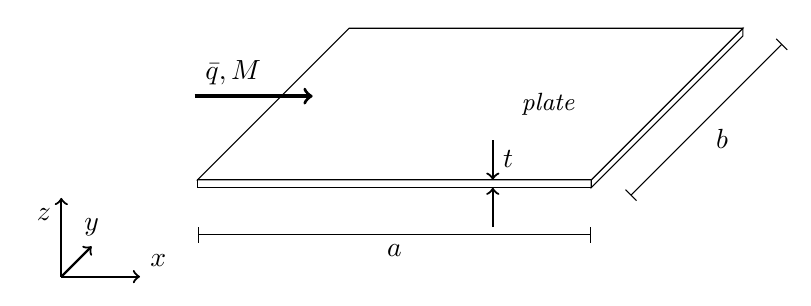
\begin{tikzpicture}
        \draw[thick,->] (-5,-2,-2)  ++(0, 0, 0) -- ++(1, 0, 0) node[anchor=south west] {$x$};
        \draw[thick,->] (-5,-2,-2)  ++(0, 0, 0) -- ++(0, 1, 0) node[anchor=north east] {$z$};
        \draw[thick,->] (-5,-2,-2)  ++(0, 0, 0) -- ++(0, 0, -1) node[anchor=south] {$y$};

        \pgfmathsetmacro{\cubex}{5}
        \pgfmathsetmacro{\cubey}{0.1}
        \pgfmathsetmacro{\cubez}{5}
        
        % \draw[black, fill=white] (2.5,0,0) ++(-\cubex/2+0.25,-\cubey-0.01,0) ++(-0.5,-0.5,0) rectangle ++(0.5,0.5,0);
        % \draw[black, fill=white] (2.5,0,0) ++(-\cubex/2+0.75,-\cubey-0.01,0) ++(-0.5,-0.5,0) -- ++(0.5,0.5,0);
        
        \draw[black, fill=white] (2.5,0,0) -- ++(-\cubex,0,0) -- ++(0,-\cubey,0) -- ++(\cubex,0,0) -- cycle;
        \draw[black, fill=white] (2.5,0,0) -- ++(0,0,-\cubez) -- ++(0,-\cubey,0) -- ++(0,0,\cubez) -- cycle;
        \draw[black, fill=white] (2.5,0,0) -- ++(-\cubex,0,0) -- ++(0,0,-\cubez) -- ++(\cubex,0,0) -- cycle;
        
        \draw[black, |-|] (2.5,-0.7,0) ++(0,0,0) -- ++(-\cubex/2,0,0)node[anchor=north] {$a$} -- ++(-\cubex/2,0,0);
        \draw[black, |-|] (3,-0.2,0) ++(0,0,0) -- ++(0,0,-\cubez/2)node[anchor=north west] {$b$} -- ++(0,0,-\cubez/2);
        
        \draw[black, thick,->] (2.5,0,0)  ++(-\cubex/4,0.5,0)node[anchor=north west]{$t$} -- ++(0,-0.5,0);
        \draw[black, thick,->] (2.5,0,0)  ++(-\cubex/4,-0.5-\cubey,0) -- ++(0,0.5,0);
        
        \draw[black, very thick, ->] (-3.5,0.1,-2.5) ++(0, 0, 0) node[anchor=south west] {$\bar{q}, M$} -- ++(1.5, 0, 0);
        
        % \draw (-1,-.4,0)node[]{\small \emph{stringer}};
        \draw (1,0,-2.5)node[]{\small \emph{plate}};
    \end{tikzpicture}
    \newline
    \caption{Panel dimensions and conditions.}
    \label{fig:problem}
\end{figure}

\subsection{Mathematical formulation}

The aerodynamic theory is a third-order Piston Theory developed by \citet{ashley_piston_1956}. As shown by \cite{pegado_metodo_2003} the Piston Theory is given by Eq.~\ref{eq:pistonTheory}, and it's third-order expansion is
given by Eq.~\ref{eq:pistonTheoryThird}.

\begin{equation}
p = p_{\infty}\Bigg[1+\frac{\gamma_{air} - 1}{2 a_{\infty}}\bigg(\frac{\partial W}{\partial t} + U_{\infty}\frac{\partial W}{\partial x}\bigg)\Bigg]^{\frac{2\gamma_{air}}{\gamma_{air}-1}}
    \label{eq:pistonTheory}
\end{equation}

\begin{equation}
p - p_{\infty} = \frac{2\bar{q}}{M}
\Bigg[
\bigg(\frac{1}{U_{\infty}}
\frac{\partial W}{\partial t} + \frac{\partial W}{\partial x}\bigg)
+
\frac{\gamma_{air}+1}{4}M
\bigg(\frac{1}{U_{\infty}}
\frac{\partial W}{\partial t} + \frac{\partial W}{\partial x}\bigg)^2
+
\frac{\gamma_{air}+1}{12}M^2
\bigg(\frac{1}{U_{\infty}}
\frac{\partial W}{\partial t} + \frac{\partial W}{\partial x}\bigg)^3
\Bigg]
    \label{eq:pistonTheoryThird}
\end{equation}

Where $p$ is the aerodynamic pressure in the surface of the plate, $p_{\infty}$ is the aerodynamic pressure of the undisturbed flow, $\gamma_{air}$ is the ratio of the air specific heat constants, $U_{\infty}$ is the velocity of the undisturbed flow, $a_{\infty}$ is the velocity of sound in the undisturbed flow and $W$ is the vertical plate displacement.

\subsection{Numerical modeling}

The aerodynamic panel is discretized in chord-wise elements \emph{CAERO5} with element property \emph{PAERO5}, each element has user defined number of span-wise strips, as illustrated in Fig. \ref{fig:problem-discrete}. 

\input{sections/model-discrete.tex}

Aerodynamic and structural models can be linked through a surface spline \emph{SPLINE1} or linear spline \emph{SPLINE2} elements.
\citet{siemens_nx_2014} indicates that rigid chord condition must be satisfied for the splines, so attachment flexibility is not allowed.
It must be specified the number of aerodynamic elements for the geometry and which set of structural nodes will be interpolated through the spline for each aerodynamic element.

As part of the solution sequence, it must be specified the parameter to run a modal analysis, which consist of the number of modes to search, the range of frequencies and the method.

It also must be specified the solution method for the aeroelastic sequence. The currently available methods are the \emph{K}, \emph{KE}, \emph{PK} and the \emph{PK-NL}, the last two are the most common used.

The flow conditions must be specified for Mach numbers, velocities and air densities, also the analysis properties of reduced frequencies and the thickness integrals corresponding the shape of the panel cross section. The values of Mach of known good correspondence of the used aerodynamic theory are $2.5 < M < 5$. To simulate a gap under the plane (no air flow) is used a air density ratio of $\frac{1}{2}$.
\cite{siemens_nx_2014}

\subsection{Solution Sequence}

Having the structural model ready and defined the problem set, the user is prompted in the Femap's interface to insert the corners of the aerodynamic panel, the number of elements span-wise and chord-wise and the structural grid nodes for each aerodynamic element.
% The model is shown at the Fig.\ref{fig:model}.

% \begin{figure}[h!]
%     \centering
%     \includegraphics[scale=0.5]{figures/undef model.png}
%     \caption{FEM model.}
%     \label{fig:model}
% \end{figure}

The the aeroelastic solution card is generated and executed in the NASTRAN solver.
The results are then plotted in \emph{Vg} and \emph{Vf} graphics for each mode, as well the complex eigenvalues.
The result set is imported in Femap, enabling the visualization of the result.

\section{RESULTS}

As proof of concept the software was utilized in a simple supported flat square plate, to reproduce the example problem \emph{HA145HA} given in \citet{siemens_nx_2014}.
The analysis was made with a 10x10 structural and aerodynamic mesh. The structural model can be visualized in Fig. \ref{fig:model}

\begin{figure}[h!]
    \centering
    \includegraphics[scale=0.5]{figures/undef-model.png}
    \caption{FEM model.}
    \label{fig:model}
\end{figure}

The \emph{Vg} plot in Fig.\ref{fig:plot} indicates the flutter condition at mode 2 and mode 17 at 607 m/s and 741 m/s, respectively.

\begin{figure}[ht]
    \centering
    \includegraphics[scale=0.8]{figures/vfvg.png}
    \caption{Vg and Vf graphics for the critical modes 2 and 17.}
    \label{fig:plot}
\end{figure}

Using the Femap's interface is possible to visualize a animated model of most critical condition (mode 2 at 607 m/s), as indicated in Fig.\ref{fig:deform}.

\begin{figure}[ht]
    \centering
    \includegraphics[scale=0.5]{figures/animated-model.png}
    \caption{Animated model view on Femap.}
    \label{fig:deform}
\end{figure}

% \begin{figure}[h!]
%     \centering
%     \includegraphics[scale=0.5]{figures/undef model.png}
%     \caption{FEM model.}
%     \label{fig:model}
% \end{figure}

% The expected results of the numerical analysis are a greater critical point of the stiffened configurations
% over the conventional configurations.
% %The boundary conditions and Mach number should have less influence in the critical point.
% The correlation of data with the literature is expected to be good, as the conditions applied
% on the numerical model are in the validity range of the linear model.

% The work of \citet{pacheco_finite_2018} has a analyzed a flat rectangular plate reinforced by a flexible beam.
% The results reached that ...

\section{CONCLUSION}

As the relevance of supersonic aerospace applications is growing, the need for more data and analysis on
related phenomena in more complex and bigger problems are increasing. The presented work interfaces with the Femap NX NASTRAN,
a broadly diffused and accepted commercial FEA software in the aerospace industry, to enable a fast and flexible pre-processing and post-processing of supersonic panel flutter problems.
This software enables the quick setup of aerodynamic model on more complex structures and other kinds phenomena (e.g.,\ curved panels, aerothermoelasticity, aeroservoelasticity),
as also for reliable and \emph{industrial-ready} design and analysis
of skin, shells and plates structures.

The software can also be improved with little effort to support others aeroelastic theories and solution sequences available in NASTRAN (e.g.,\ strip theory, aeroelastic response, model sensibility and optimization).

The software may be made available given a reasonable request.


\section{REFERENCES} 

\bibliographystyle{abcm}
\renewcommand{\refname}{}
\bibliography{references}

The authors are the only responsible for the printed material included in this paper.

\end{document}
